\chapter{Function Handles and Zero-Finding}
\label{fzero}

In this chapter we'll learn how to use \emph{function handles} to pass a function to a MATLAB solver such as the MATLAB function \lstinline{fzero}.   This is a common technique we'll see later in applications of numerically solving differential equations and performing optimizations.

To demonstrate the technique we'll the MATLAB function \lstinline{fzero} to solve nonlinear equations.
Nonlinear equations are useful for modeling physical systems; for example, in one of
the exercises at the end of this chapter, you can use \lstinline{fzero} to find the equilibrium point of an object floating on water.

\section{Solving Nonlinear Equations}

\index{nonlinear equation}
\index{equation!nonlinear}

What does it mean to ``solve'' an equation?  That may seem like an
obvious question, but let's take a minute to think about it,
starting with a simple \mbox{example}.

Suppose we want to know the
value of a variable, $x$, but all we know about it is the relationship
$x^2 = a$. If you've taken algebra, you probably  know how to solve this
equation: you take the square root of both sides and get
$x = \pm \sqrt{a}$.  Then, with the satisfaction of a job well done,
you move on to the next problem.

\index{square root}

But what have you really done?  The relationship you derived is
equivalent to the relationship you started with---they contain the
same information about $x$---so why is the second one preferable
to the first?

There are two reasons.  One is that the relationship is now \emph{explicit} in $x$: because $x$ is all alone on the left side, we can treat the right side as a recipe for computing $x$, assuming that we know the value of $a$.

\index{explicit computation}
\index{computation!explicit}

The other reason is that the recipe is written in terms of operations
we know how to perform.  Assuming that we know how to compute square
roots, we can compute the value of $x$ for any value of $a$.

When people talk about solving an equation, what they usually mean
is something like ``finding an equivalent relationship that is
explicit in one of the variables.''  In the context of this book,
that's what we'll call an \emph{analytic \mbox{solution}}, to distinguish
it from a \emph{numerical solution}, which is what we are going to
do next.

\index{analytic solution}
\index{numerical solution}

{\binoppenalty=\maxdimen%
\relpenalty=\maxdimen% [keeps the equation from being broken across lines]
To demonstrate a numerical solution, consider the equation 
\begin{equation} \label{e:fzero}
x^2 - 2x = 3.
\end{equation}  
You could solve this analytically, either by factoring it or by
using the quad\-ratic formula, and you would discover that there are
two solutions, $x=3$ and $x=-1$.  Alternatively, you could solve it
numerically by rewriting it as $x = \pm \sqrt{2x+3}$.}

This equation is not explicit, since $x$ appears on both sides, so
it's not clear that this move did any good at all.  But suppose we had
reason to expect a solution near 4.
We could start with $x=4$ as an \emph{initial value} and then use
the equation $x = \sqrt{2x+3}$ to compute successive
approximations of the solution. (To understand why this
works, see \url{https://greenteapress.com/matlab/fixed}.)

\index{fixed-point iteration}

Here's what happens:

\begin{code}
>> x = 4;
>> x = sqrt(2*x+3)
x = 3.3166

>> x = sqrt(2*x+3)
x = 3.1037

>> x = sqrt(2*x+3)
x = 3.0344

>> x = sqrt(2*x+3)
x = 3.0114

>> x = sqrt(2*x+3)
x = 3.0038
\end{code}

After each iteration, \lstinline{x} is closer to the correct answer,
and after five iterations the relative error is about 0.1 percent, which
is good enough for most purposes.

\index{numerical method}

Techniques that generate numerical solutions are called
\emph{numerical \mbox{methods}}.
The nice thing about the method we just used is that it's simple.  But it doesn't always
work, and it's not often used in practice.
We'll see a better alternative in the next section.

\subsection{Zero-Finding}
\label{zero}

\index{zero-finding}
\index{error function}
\index{function!error}

The MATLAB function \lstinline{fzero} that uses numerical methods to search for solutions to nonlinear equations. The documentation of the \lstinline{fzero} starts with
\begin{stdout}
fzero  Single-variable nonlinear zero finding. 
    X = fzero(FUN,X0) tries to find a zero of the function FUN near X0, 
    if X0 is a scalar. 
\end{stdout}
which tells us we need to pass in the function \mcode{FUN} as the first argument to the \mcode{fzero} tool.
In order to do this, we have to rewrite Eq.~(\ref{e:fzero}) as an \emph{error function},
\begin{equation*}
f(x) = x^2 - 2x -3,
\end{equation*}
and pass that function to \mcode{fzero} as a \emph{function handle}.

The value of the error function is 0 if $x$ is a solution and nonzero if it is not.
This function is useful because we can use values of $f(x)$, evaluated at various values of $x$, to infer the location of the solutions.  And that's what \lstinline{fzero} does.
Values of $x$ where $f(x) = 0$ are called zeros of the function or \emph{roots}.

\index{root}
\index{fzero@\lstinline{fzero}}

To use \lstinline{fzero} you have to define a MATLAB function that computes the error function, like this:
\begin{code}
function res = error_func(x)
    res = x^2 - 2*x -3;
end
\end{code}
The classical way of defining this function 

You can call \lstinline{error_func} from the Command Window and confirm that $3$ and $-1$ are zeros:

\begin{code}
>> error_func(3)
ans = 0

>> error_func(-1)
ans = 0
\end{code}

But let's pretend that we don't know where the roots are; we only know that one of them is near 4.  Then we could call \lstinline{fzero} like this:

\begin{code}
>> fzero(@error_func, 4)
ans = 3.0000
\end{code}

Success!  We found one of the zeros.

The first argument is a \emph{function handle} that specifies
the error function.  The \lstinline{@} symbol allows us to name the
function without calling it.  The interesting thing here is
that you're not actually calling \lstinline{error_func} directly;
you're just telling \lstinline{fzero} where it is.  In turn, \lstinline{fzero}
calls your error function---more than once, in fact.

\index{function handle}
\index{handle!function}

The second argument is the initial value.  If we provide a different
value, we get a different root (at least sometimes).

\begin{code}
>> fzero(@error_func, -2)
ans = -1
\end{code}

Alternatively, if you know two values that bracket the root,
you can provide both.

\begin{code}
>> fzero(@error_func, [2,4])
ans = 3
\end{code}

The second argument is a vector that contains two elements.

\index{vector}

You might be curious to know how many times \lstinline{fzero} calls your
function, and where.  If you modify \lstinline{error_func} so that it displays
the value of \lstinline{x} when it is called and then run \lstinline{fzero}
again, you get

\begin{code}
>> fzero(@error_func, [2,4])
x = 2
x = 4
x = 2.75000000000000
x = 3.03708133971292
x = 2.99755211623500
x = 2.99997750209270
x = 3.00000000025200
x = 3.00000000000000
x = 3
x = 3
ans = 3
\end{code}

Not surprisingly, it starts by computing $f(2)$ and $f(4)$.  Then it computes a point in the interval, $2.75$, and evaluates $f$ there.  After each iteration, the interval gets smaller, and the guess gets closer to the true root.
The \lstinline{fzero} function stops when the interval is so small that the estimated
zero is correct to about 15~digits.

If you'd like to know more about how \lstinline{fzero} works, see Chapter~\ref{howfzero}.


\subsection{What Could Go Wrong?}

The most common problem people have with \lstinline{fzero} is leaving
out the \lstinline{@}.  In that case, you get something like so:

\begin{code}
>> fzero(error_func, [2,4])
Not enough input arguments.

Error in error_func (line 2)
    res = x^2 - 2*x -3;
\end{code}

The error occurs because MATLAB treats the first argument as a function call, so it calls \lstinline{error_func} with no arguments.

\index{output variable}
\index{variable!output}

Another common problem is writing an error function that never
assigns a value to the output variable.  In general, functions should
\emph{always} assign a value to the output variable, but MATLAB doesn't
enforce this rule, so it's easy to forget.

For example, if you
write

\begin{code}
function res = error_func(x)
    y = x^2 - 2*x -3
end
\end{code}
and then call it from the Command Window,
\begin{code}
>> error_func(4)
y = 5
\end{code}
it looks like it worked, but don't be fooled.  This function assigns
a value to \lstinline{y}, and it displays the result, but when the function
ends, \lstinline{y} disappears along with the function's workspace.
If you try to use it with \lstinline{fzero}, you get

\begin{code}
>> fzero(@error_func, [2,4])
y = -3

Error using fzero (line 231)
FZERO cannot continue because user-supplied function_handle ==>
error_func failed with the error below.

Output argument "res" (and maybe others) not assigned during call
to "error_func".
\end{code}

If you read it carefully, this is a pretty good error message,
provided you understand that ``output argument'' and ``output variable'' are the same thing.

\index{argument}
\index{output argument}

You would have seen the same error message when calling \lstinline{error_func} from the interpreter, if you had assigned the result to a variable:

\begin{code}
>> x = error_func(4)
y = 5

Output argument "res" (and maybe others) not assigned during
call to "error_func".
\end{code}

Another thing can go wrong: if you provide an interval for the
initial guess and it doesn't actually contain a root, you get

\begin{code}
>> fzero(@error_func, [0,1])
Error using fzero (line 272)
The function values at the interval endpoints must differ in sign.
\end{code}

\index{interval}

There is one other thing that can go wrong when you use \lstinline{fzero}, but
this one is less likely to be your fault.  It's possible that \lstinline{fzero}
won't be able to find a root.

Generally, \lstinline{fzero} is robust, so you may never have a problem, but you should remember that there is no guarantee that \lstinline{fzero} will work, especially  if you provide a single value as an initial guess.  Even if you provide an interval that brackets a root, things can still go wrong if the error function is discontinuous.


\subsection{Choosing an Initial Value}

The better your initial value is, the more likely it is that
\lstinline{fzero} will work, and the fewer iterations it will
need.

When you're solving problems in the real world, you'll usually
have some intuition about the answer.  This intuition is often enough
to provide  a good initial guess.

If not, another way to choose an initial guess is to plot the error function and
approximate the zeros visually.  Here is a short script to do just that:

\lstinputlisting[style=mcode]{../code/chap_zerofinding/plot_error.m}

We've used the \lstinline{linspace} command to create a vector starting at -2, ending with 5, with 100 elements. The \lstinline{grid on} command displays the gray grid lines, which help identify the zero crossings.  You may also notice that if you use by hovering the cursor over the graph, MATLAB will display the nearest data point values using the \emph{data tips} interactive tool, illustrated in Figure~\ref{f:error_data}

\begin{figure}[h]
    \centerline{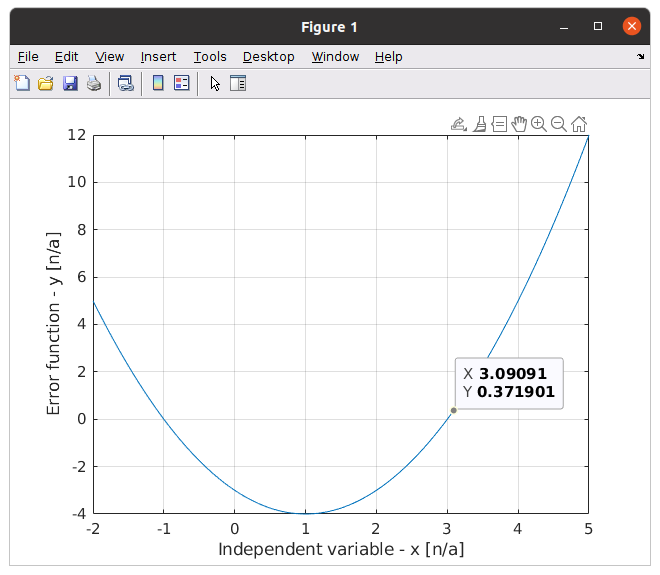
\includegraphics[width=0.7\textwidth]{images/error_w_data.png}}
    \caption{Visualization of the error function.}
    \label{f:error_data}
\end{figure}


    \subsection{Vectorizing Functions}

\index{vectorizing}
\index{function!vectorizing}

When you call the plotting script, you might get the following warning:

\begin{stdout}
Error using  ^ 
Incorrect dimensions for raising a matrix to a power. Check that the matrix
is square and the power is a
scalar. To operate on each element of the matrix individually, 
use POWER (.^) for elementwise power.
Error in error_func (line 2)
    res = x^2 - 2.*x -3;
Error in plot_error (line 3)
y = error_func(x); 
\end{stdout}

This means that MATLAB tried to call \lstinline{error_func} with a vector, and it failed.
The problem is that it uses the \lstinline{*} and \lstinline{^} operators which refer to matrix operations that follow the rules of linear algebra.  In this case this is not what we intended; instead we want to do \emph{element-wise} array multiplication and exponentiation (see ``\nameref{elementwise}'' on page~\pageref{elementwise}).

\index{element-wise operator}
\index{operator!element-wise}

If you rewrite \lstinline{error_func} like this:

\begin{code}
function res = error_func(x)
    res = x.^2 - 2.*x -3;
end
\end{code}
the warning message goes away.

\subsection{Anonymous Functions}

One way to avoid a separate M-file, \emph{error\_func.m}, for the function definition we provide to \lstinline{fzero} is to define an 
\href{https://www.mathworks.com/help/matlab/matlab_prog/anonymous-functions.html}{\emph{anonymous function}}.  
An anonymous function is a single statement function, not stored in a separate program file, associated with a function handle.  

\lstinputlisting[style=mcode_numbers]{../code/chap_zerofinding/fzero_afunc.m}

The second line defines the singe-expression anonymous function handle, \lstinline{error_afunc_handle}.  Then we pass the function handle to \lstinline{fzero}.  Note that the \lstinline{error_afunc_handle} variable stores a function handle - not a function.
\begin{code}
    >> whos
  Name                    Size            Bytes  Class              Attributes

  ans                     1x1                 8  double                       
  error_afunc_handle      1x1                32  function_handle    
\end{code}
This is the reason why there is no \lstinline{@} in the call to \lstinline{fzero}.

Anonymous function make the code more concise, avoiding having separate files for script and the function definition, but at the expense of readability.  Among other issues, the syntax for defining anonymous functions is less-than intuitive.  A better way of being concise while maintaining readability might be to use a local function.  Since R2024a, local functions can be anywhere in the script file, not just at the end, so an equivalent implementation would be...

\lstinputlisting[style=mcode_numbers]{../code/chap_zerofinding/fzero_demo_local.m}

It is still beneficial to be aware of anonymous functions.  You will likely run into online examples and documentation that uses anonymous functions, even if you don't write them yourself.

\section{How fzero Works}
\label{howfzero}

According to the MATLAB documentation, \lstinline{fzero} uses ``a combination of bisection, secant, and inverse quadratic interpolation methods.''  (See \url{https://greenteapress.com/matlab/fzero})

\index{fzero@\lstinline{fzero}}
\index{bisection}
\index{secant method}
\index{inverse quadratic interpolation}
\index{root}

To understand what that means, suppose we're trying to find a root of a function of one variable, $f(x)$, and assume we have evaluated the function at two places, $x_1$ and $x_2$, and found that the results have opposite signs.  Specifically, assume $f(x_1) > 0$ and $f(x_2) < 0$, as shown in Figure~\ref{fig:secant}.

\begin{figure}[h]
\centerline{\includegraphics[scale=0.8]{images/figure15_03_new.eps}}
\caption{Initial state of a root-finding search}
\label{fig:secant}
\end{figure}

As long as $f$ is continuous, there must be at least one root in this interval.
In this case we would say that $x_1$ and $x_2$ \emph{bracket} a zero.

\index{bracket}

If this were all you knew about $f$, where would you go looking for
a root?  If you said ``halfway between $x_1$ and $x_2$,''
congratulations!  You just invented a numerical method called
\emph{bisection}!

If you said, ``I would connect the dots with a straight line
and compute the zero of the line,''
congratulations!  You just invented the \emph{secant method}!

And if you said, ``I would evaluate $f$ at a third point, find the
parabola that passes through all three points, and compute the zeros
of the parabola,'' congratulations, you just invented
\emph{inverse quadratic interpolation}!

That's most of how \lstinline{fzero} works.  The details of how these methods are combined are interesting, but beyond the scope of this book.  You can read more at \url{https://greenteapress.com/matlab/brent}.




\section{Debugging}

When you start writing longer programs, you might spend more time debugging.  So we'll end this chapter with some debugging tips.

\subsection{More Name Collisions}

Functions and variables occupy the same workspace, which means
that whenever a name appears in an expression, MATLAB starts by looking
for a variable with that name; if there isn't one, it looks for
a function.

\index{name collision}
\index{collision!name}
\index{shadow}

As a result, if you have a variable with the same name as a function,
the variable \emph{shadows} the function; metaphorically, you can't see the function because the variable is in the way.

For example, if you assign
a value to \lstinline{sin} and then try to use the \lstinline{sin} function, you
might get an error:

\begin{code}
>> sin = 3;
>> sin(5)
Index exceeds the number of array elements (1).

'sin' appears to be both a function and a variable.
If this is unintentional, use 'clear sin' to remove
the variable 'sin' from the workspace.
\end{code}

Since the value we assigned to \lstinline{sin} is a number, and a number is considered a $1 \times 1$ matrix, MATLAB tries to access the fifth element of the matrix and finds that there isn't one.

In this case, MATLAB is able to detect the error, and the error message is pretty helpful.
But if the value of \lstinline{sin} were a vector, or if the argument were smaller, you would be in trouble.  For example,

\begin{code}
>> sin = 3;
>> sin(1)
ans = 3
\end{code}

Just to review, the sine of 1 is not 3!

You can avoid these problems by choosing function names carefully. Use long, descriptive names for functions, not single letters like \lstinline{f}. To be even clearer, use function names that end in \lstinline{func}. And before you define a function, check whether MATLAB already has a function with the same name.

\subsection{Debugging Your Head}

When you're working with a new function or a new language feature
for the first time, you should test it in isolation before you
put it into your program.

\index{debugging}

For example, suppose you know that \lstinline{x} is the sine of some
angle and you want to find the angle.  You find the MATLAB function
\lstinline{asin}, and you're pretty sure it computes the inverse sine
function.  Pretty sure is not good enough; you want to be very sure.

Since we know $\sin 0 = 0$, we could try

\begin{code}
>> asin(0)
ans = 0
\end{code}
which is correct.  Now, we also know that the sine of $90$\textdegree is
1, so if we try \lstinline{asin(1)}, we expect the answer to be 90, right?

\begin{code}
>> asin(1)
ans = 1.5708
\end{code}

Oops.  We forgot that the trig functions in MATLAB work in radians,
not degrees.  The answer we got is $\pi/2$, which is $90$\textdegree, in radians.

With this kind of testing, you're not really checking for
errors in your program; you're checking your understanding.  If you
make an error because you are confused about how MATLAB works, it
might take a long time to find, because when you look at the code,
it looks right.

\index{debugging!Seventh Theorem}

Which brings us to the Seventh Theorem of Debugging:

\begin{quote}
The worst bugs aren't in your code; they're in your head.
\end{quote}

\section{Chapter Review}

This chapter introduced \lstinline{fzero}, a function we can use to solve nonlinear equations.
To use \lstinline{fzero}, you have to write an error function and pass a function handle as an argument.  Using functions in this way can be tricky at first, but get comfortable with it, because we are going to use it a lot.

Here are some terms from this chapter you might want to remember.

If we can solve an equation by performing algebraic operations and deriving an explicit way to compute a value, the result is an \emph{analytic solution}.
Otherwise, we can use a \emph{numerical method}, which finds a \emph{numerical solution} to the equation, which is usually an approximation.

To solve nonlinear equations, we often rewrite them as functions and then find one or more \emph{zeros} of the function, that is, arguments that make the value of the function $0$.

A \emph{function handle} is a way of
referring to a function by name (and passing it as an argument)
without calling it.

A \emph{anonymous function} is a single-expression function definition, not defined in its own separate file, where the resulting function handle is assigned to a variable.

Finally, \emph{shadowing} is a kind of name collision in which a new definition
causes an existing definition to become invisible.  In MATLAB,
variable names can shadow built-in functions (with hilarious results).

In the next chapter, we'll write functions that take vectors as inputs and return vectors as outputs.


\section{Exercises}

Before you go on, you might want to work on the following exercises.

\begin{ex}

\begin{enumerate}

\index{Chebyshev polynomial}

\item Write a function called \lstinline{cheby6} that evaluates the
sixth Chebyshev polynomial.  It should take an input variable,
$x$, and return

\begin{equation*}
32 x^6 - 48 x^4 + 18 x^2 - 1
\end{equation*}

\item Use \lstinline{plot} to display a graph of this function in the
interval from $-1$ to $1$.  Estimate the location of any zeros in this
range.

\item Use \lstinline{fzero} to find as many different roots as you can.
Does \lstinline{fzero} always find the root that is closest to the initial
value?

\end{enumerate}

% cheby6.m
\end{ex}


\begin{ex}
\label{ex:duck}

When a duck is floating on water, how much of its body is submerged?\footnote{This exercise is adapted from C.~F.~Gerald and P.~O.~Wheatley, \emph{Applied Numerical Analysis}, 4th edition (Boston: Addison-Wesley, 1989).}

\index{duck}
\index{sphere}

To estimate a solution to this problem, we'll assume that the submerged part of a duck is well approximated by a section of a sphere.
If a sphere with radius $r$ is submerged in water to a depth $d$, the
volume of the sphere below the water line is

\[ V = \frac{\pi}{3} (3r d^2 - d^3) \quad
\mbox{as long as} \quad d < 2 r  \]

We'll also assume that the density of a duck is $\rho = 0.3$\,g/cm$^3$ (0.3 times the density of water) and that its mass is $\frac{4}{3} \pi r^3 \rho$\,g.

Finally, according to the law of buoyancy, an object floats at the level where the weight of the displaced water equals the total weight of the object.

\index{density}
\index{buoyancy}

Here are some suggestions for how to proceed:

\begin{enumerate}

\item Write an equation relating $\rho$, $d$, and $r$.

\item Rearrange the equation so the right-hand side is zero.
Our goal is to find values of $d$ that are roots of this equation.

\item Write a MATLAB function that evaluates this function.  Test it,
   then make it a quiet function.

\item Make a guess about the value of $d_0$ to use as an initial value.

\item Use \lstinline{fzero} to find a root near $d_0$.

\item Check to make sure the result makes sense.  In particular,
   check that $d < 2 r$, because otherwise the volume equation
   doesn't work!

\item Try different values of $\rho$ and $r$ and see if you get the
  effect you expect.  What happens as $\rho$ increases?  Goes to
  infinity?  Goes to zero?  What happens as $r$ increases?  Goes to
  infinity?  Goes to zero?

\end{enumerate}


% TODO: Find places in the book where error messages are getting syntax highlighting, and put them in a verbatim environment.


\end{ex}
